%%%%%%%%%%%%%%%%%%%%%%%%%%%%%%%%%%%%%%%%%%%%%%%%%%%%%%%%%%%%%%%%%%%%%%%%%%%%%%%%
% Results section
\chapter{Results} \label{chap:results}

% In processing the collected data, some
% technicalities
When at any point a path is incalculable due to satellite outage, the path reported is of length one (a single point at the position of the leader). When this occurs, the following distance becomes 0.0, and these instances were ignored in examination of data runs. Refer to Apps. \ref{app:precisionresults} and \ref{app:zeroresults} for timeseries data and alert frequency in the precision following and zero landmark tests.

Rearranging Eq.~\eqref{eq:stopdist} to solve for $\mu$ at every time step given the curvilinear following distance and magnitude of the follower's ground-plane velocity, as in Eq.~\eqref{eq:mureq}, yields what friction coefficient $\mu_{require}$ is necessary at any instant for the following vehicle to stop without impacting the lead vehicle.
\begin{align} \label{eq:mureq}
    \mu_{required} &= \left( \frac {1} {d g} \right) \left(\frac {|\bar{v}|^2} {2} \right)
\end{align}
Probability density functions of $\mu_{required}$ for the precision following and zero landmark tests are explained below, and given in Figs. \ref{fig:precision_mu_dist} and \ref{fig:zero_mu_dist}.


%%%%% Lane Change between Cones -  need GUI specificity
\section{Lane Change Replication Test Results} \label{sec:lanechangetestresults}

Table \ref{tab:lanechangeresults} shows the results of all runs of the lane change replication test. Figures~\ref{fig:lanechange_earth} and~\ref{fig:lanechange_mono} show what the driver saw on the screen prior to attempting to make the correct lane change using the Earth GUI and the monolithic GUI, respectively.
% Always changed lanes too late

\begin{table}[htbp] \centering \caption{Cone pairs chosen in the lane change replication test}
\begin{tabular}{rc|cc} 
    GUI&    Run \#  &     Leader&    Follower \\ \hline\hline
    Earth&      1       &       1   &    3 \\
         &      2       &       3   &    4   \\ \hline
    Monolith&   3       &       2   &    3   \\
         &      4       &       5   &    5 \\ \hline   
\end{tabular} \label{tab:lanechangeresults} \end{table}

% Accuracy of google earth stuff
As mentioned previously, the DRTK algorithm sacrifices accuracy in the global coordinate frame in favor of high accuracy in relative coordinate frames. In the case of path following, this means that at any time the current RPV to the leader from the follower will be extremely accurate. 
% TDCP accuracy
% When moving, path points will decrease in accuracy from the leader to the follower due to the time-dependent nature of TDCP accuracies.
Google Earth, on the other hand, has been found to contain errors with a mean of 19.0 m , and a standard deviation of 12.3 m~\cite{ge_accuracy}. In GNSS applications, technologies possessing errors on this scale are considering to be highly inaccurate. All points of interest (leader and all path points) are placed on the Google Earth screen by using the standalone GPS position of the follower and adding the RPV from the leader. Even ignoring the errors in standalone GPS, a 19.0 m translation from the true position would put all objects which drivers use to orient themselves well away from their true position as observed by the naked eye. However, the relative positions and scale on the Google Earth screen still remain true. This was known during the testing, but testers still reported this issue to be disconcerting when determining where to change lanes, and the resulting performance decrease as compared to the monolithic GUI is visible. In every instance (across all runs) where a lane change was made between the improper cone pair, the follower changed lanes later than did the leader. This is attributed to latency existing in the combined system from calculation and driver reaction for both GUIs.

\begin{figure}[ht] \centering
    \begin{minipage}[b]{0.45\linewidth} \centering 
        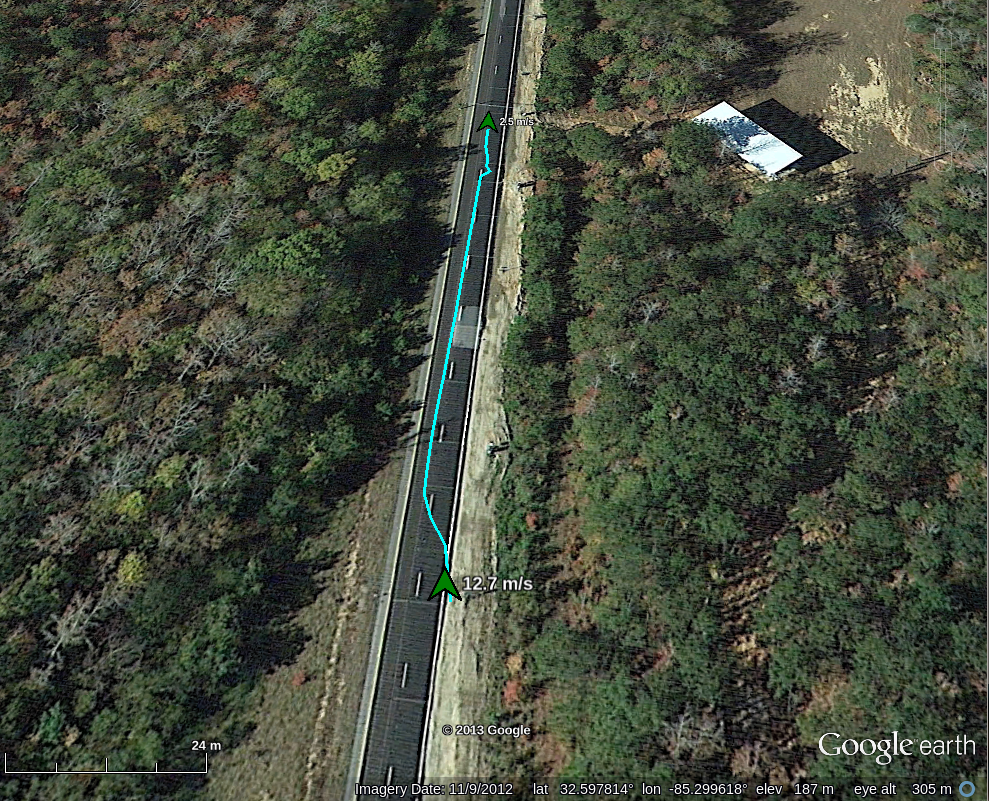
\includegraphics[width=\textwidth]{./figs/lane_change.png}
        \caption{Earth GUI as follower enters a lane change} \label{fig:lanechange_earth}
    \end{minipage}
    \hspace{0.5cm}
    \begin{minipage}[b]{0.45\linewidth} \centering
        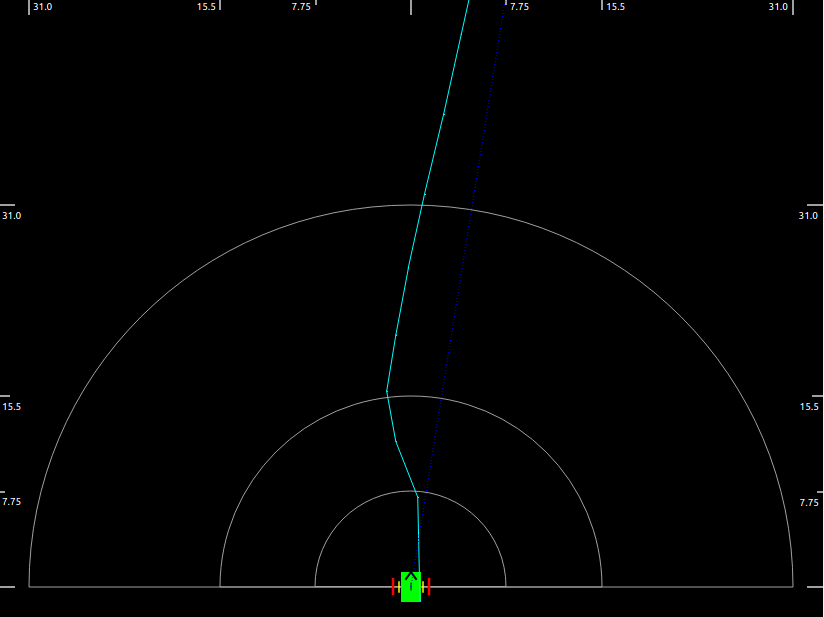
\includegraphics[width=\textwidth]{./figs/lane_change_mono.png}
        \caption{Monolithic GUI as follower enters a lane change} \label{fig:lanechange_mono}
    \end{minipage}
\end{figure}



%%%%% Follow the Path around the track
\section{Precision Following Test Results} \label{sec:precisionfollowingresults}

% Explain the run-specific charts
Shown in Figs. \ref{fig:precisionresults_earth} , \ref{fig:precisionresults_monolith} , and \ref{fig:precisionresults_control} are the best of all runs of the precision following test using the Earth-based GUI, monolithic GUI, and no GUI at all, respectively. All drivers had executed the test with at least one of the graphical tools prior to executing it without aid in the control runs, to gain an understanding of the spacing requirements. The criterion for selecting the `best' run was that which had the lowest combined percentage of timesteps when an alert was issued for either distance or deviation. Figure \ref{fig:precision_alerts} outlines how often alerts occurred during each data run.

\begin{table}[htbp] \centering \caption{Mean absolute deviation for the precision following test}
\begin{tabular}{r|c} 
    GUI&    Mean abs. dev. \\ \hline\hline
    Earth&      0.9677 m \\
    Monolith&   0.4719 m \\
    Control&    0.2069 m \\ \hline   
\end{tabular} \label{tab:precision_dev_mean} \end{table}

The Earth GUI enabled drivers to maintain spacing very close to the warning distance while going below few times. This is evidenced by the high probability density just below $\mu_{warn}$ in Fig. \ref{fig:precision_mu_dist}. Both tools totally eliminated critical distance alerts altogether, but the monolithic GUI was unsuccessfull at preventing warning distances, as the peak probability density was reached at a higher $\mu$ value than either the Earth GUI or the control.
\begin{figure}[ht] \centering % good.
    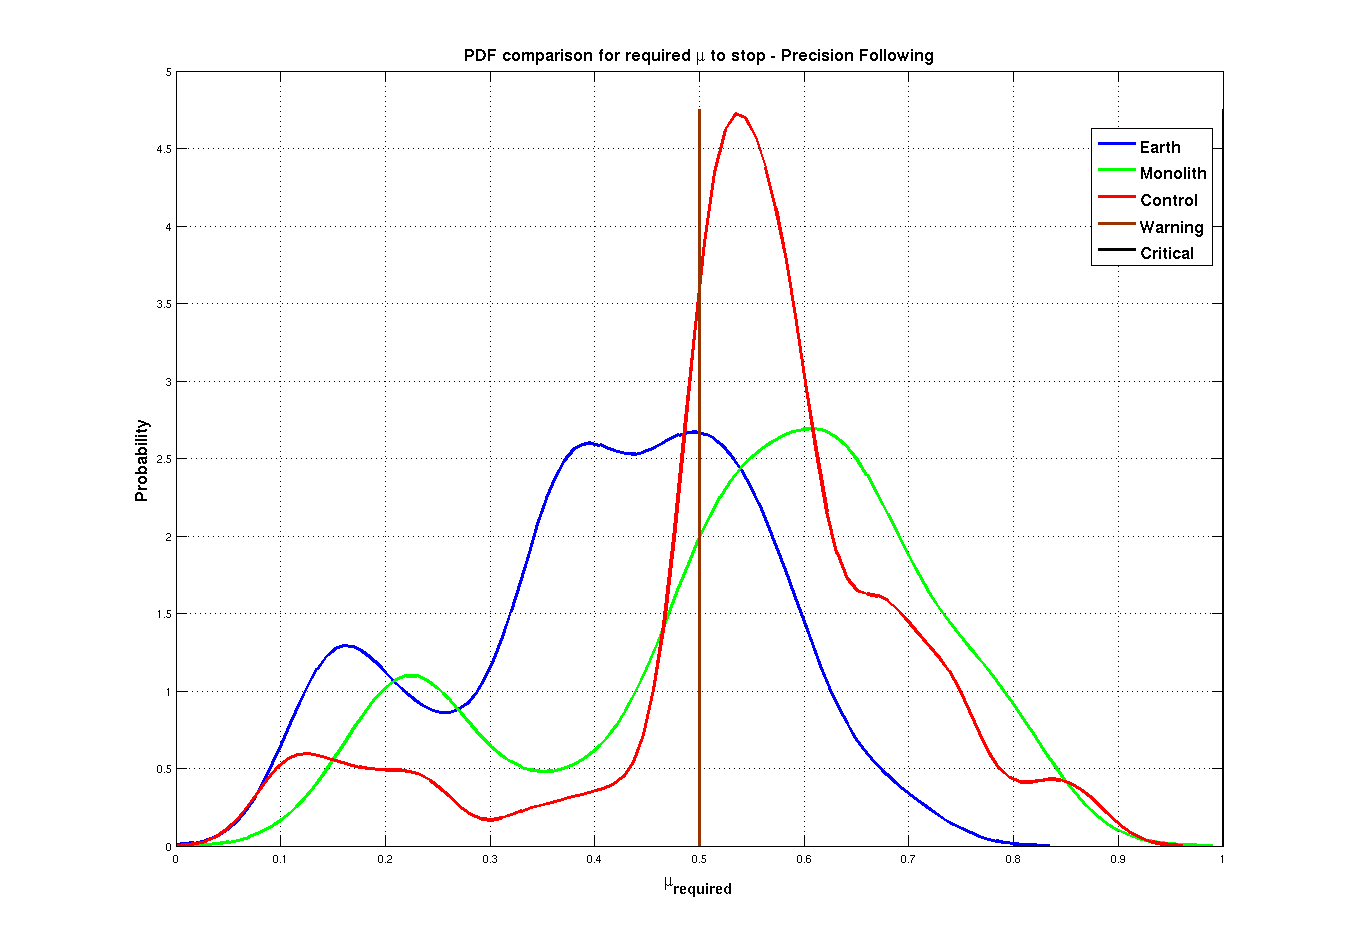
\includegraphics[width=6in]{./figs/precision_following_mu_distribution.png}
    \caption{Comparison of smoothed $\mu_{required}$ distributions for the precision following test} \label{fig:precision_mu_dist}
\end{figure}
Conversely, the monolithic GUI enabled drivers to maintain higher precision with respect to lateral path deviation, as it has a much tighter distribution about zero in Fig.~\ref{fig:precision_dev_dist}, reaching a peak right at zero, resulting in a lower mean absolute deviation as seen in Table \ref{tab:precision_dev_mean}.
\begin{figure}[ht] \centering % good.
    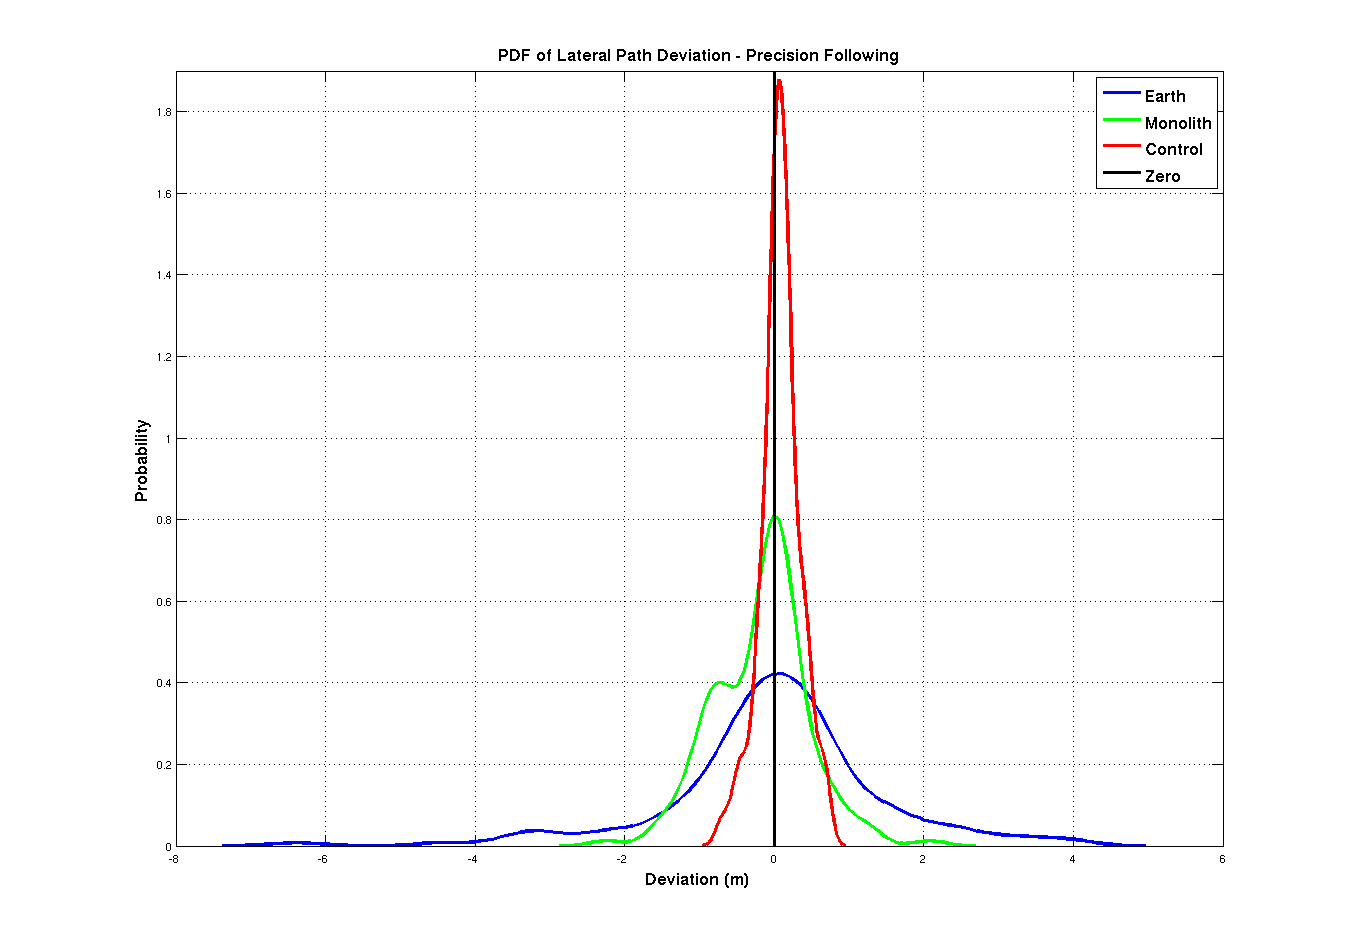
\includegraphics[width=6in]{./figs/precision_following_dev_pdf.png}
    \caption{Comparison of smoothed deviation distributions for the precision following test} \label{fig:precision_dev_dist}
\end{figure}



%%%%% Skidpad drive around
\section{Zero Landmark Test Results} \label{sec:zerolandmarkresults}

% Explain the run-specific charts
Shown in Figs. \ref{fig:zeroresults_earth} , \ref{fig:zeroresults_monolith} , and \ref{fig:zeroresults_control} are the best of all runs of the zero landmark test using the Earth-based GUI, monolithic GUI, and no GUI at all, respectively. All drivers had executed the test with at least one of the graphical tools prior to executing it without aid in the control runs, to gain an understanding of the spacing requirements. The criterion for selecting the `best' run was that which had the lowest combined percentage of timesteps when an alert was issued for either distance or deviation. Figure \ref{fig:zero_alerts} outlines how often alerts occurred during each data run.

\begin{table}[htbp] \centering \caption{Mean absolute deviation for the zero landmark test}
\begin{tabular}{r|c} 
    GUI&    Mean abs. dev. \\ \hline\hline
    Earth&      2.7404 m \\
    Monolith&   3.6830 m \\
    Control&    0.7267 m \\ \hline   
\end{tabular} \label{tab:zero_dev_mean} \end{table}

% Problems with the zero landmark test - how the contro
The goal was to deprive drivers of visual landmarks during the test, which succeeded for comparing the two GUIs since most drivers report looking at the computer screen exclusively. However, during control runs, drivers elected to stay directly behind the leading vehicle and forfeit following safety rather than to carefully attempt to replicate a path. This strategy taken in the control runs ended up producing more successful results for deviation than using the graphical tools, as seen in the mean values of absolute deviation in Table \ref{tab:zero_dev_mean}. 
\begin{figure}[ht] \centering % good.
    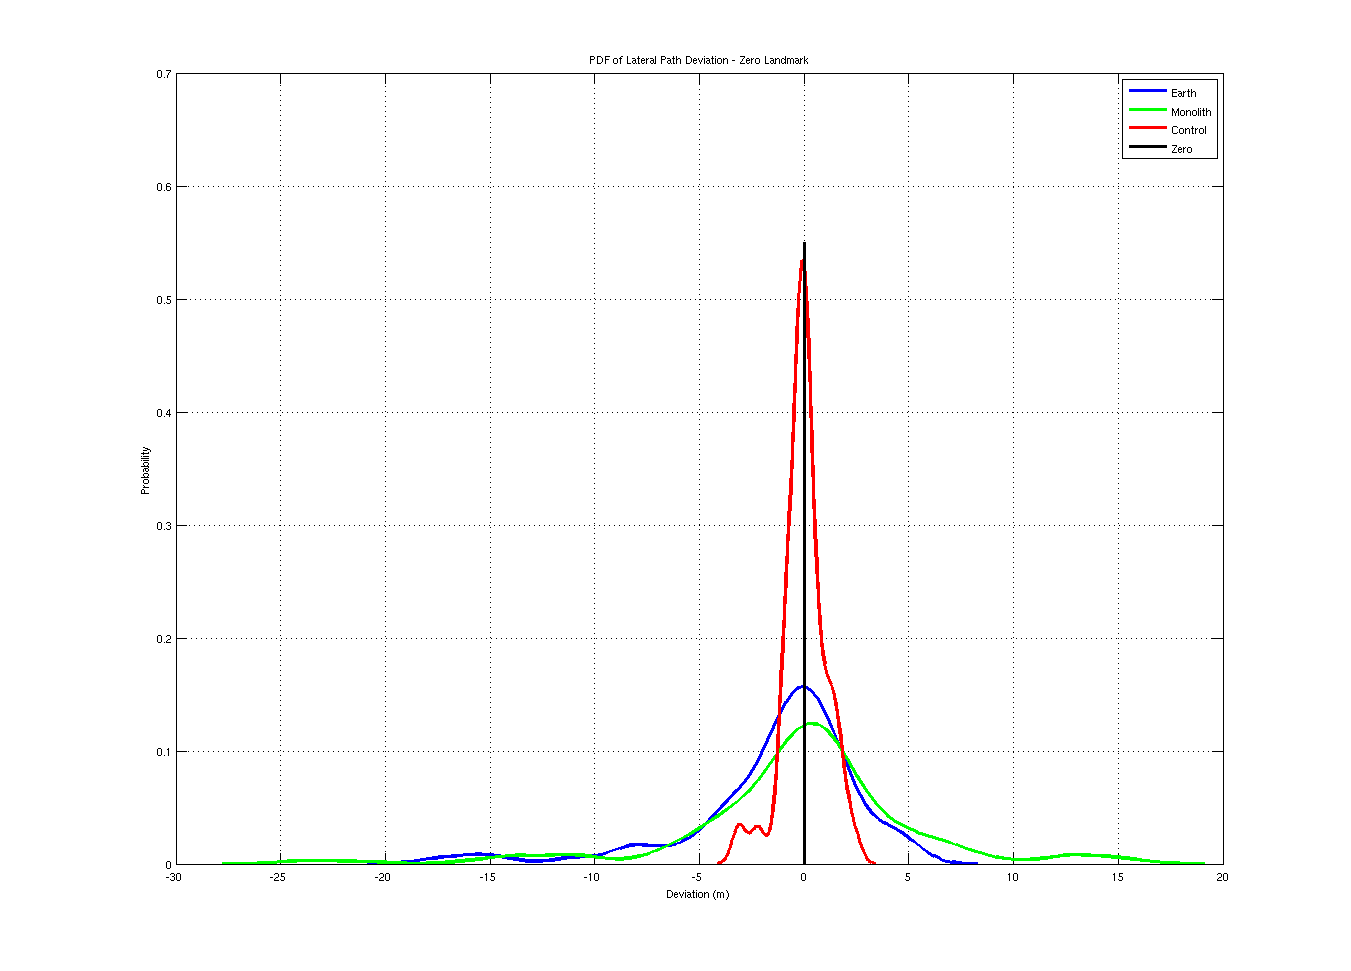
\includegraphics[width=6in]{./figs/zero_landmark_dev_pdf.png}
    \caption{Comparison of smoothed deviation distributions for the zero landmark test} \label{fig:zero_dev_dist}
\end{figure}
With no other reference, drivers were most likely to over- or under-correct for path deviations when using the visual tools, and due to lag in the system, had delayed reaction times. This resulted in a greater distribution of deviations as compared to control runs, as seen in \ref{fig:zero_dev_dist}. However, due to the radical nature of the course changes, biases were much more likely to arise (i.e., in the best control run, the driver was more likely to deviate to the left). Both GUI's were successful at eliminating this bias, resulting in probability densities of lateral deviation which were evenly distributed about zero.

% distances
Figure \ref{fig:zero_mu_dist} shows how remaining further behind the lead vehicle while using the graphical tools to replicate paths resulted in significantly lower surface friction required to stop without experiencing a rear end collision. Distance alerts were eliminated altogether when using either of the two graphical tools.
\begin{figure}[ht] \centering % good.
    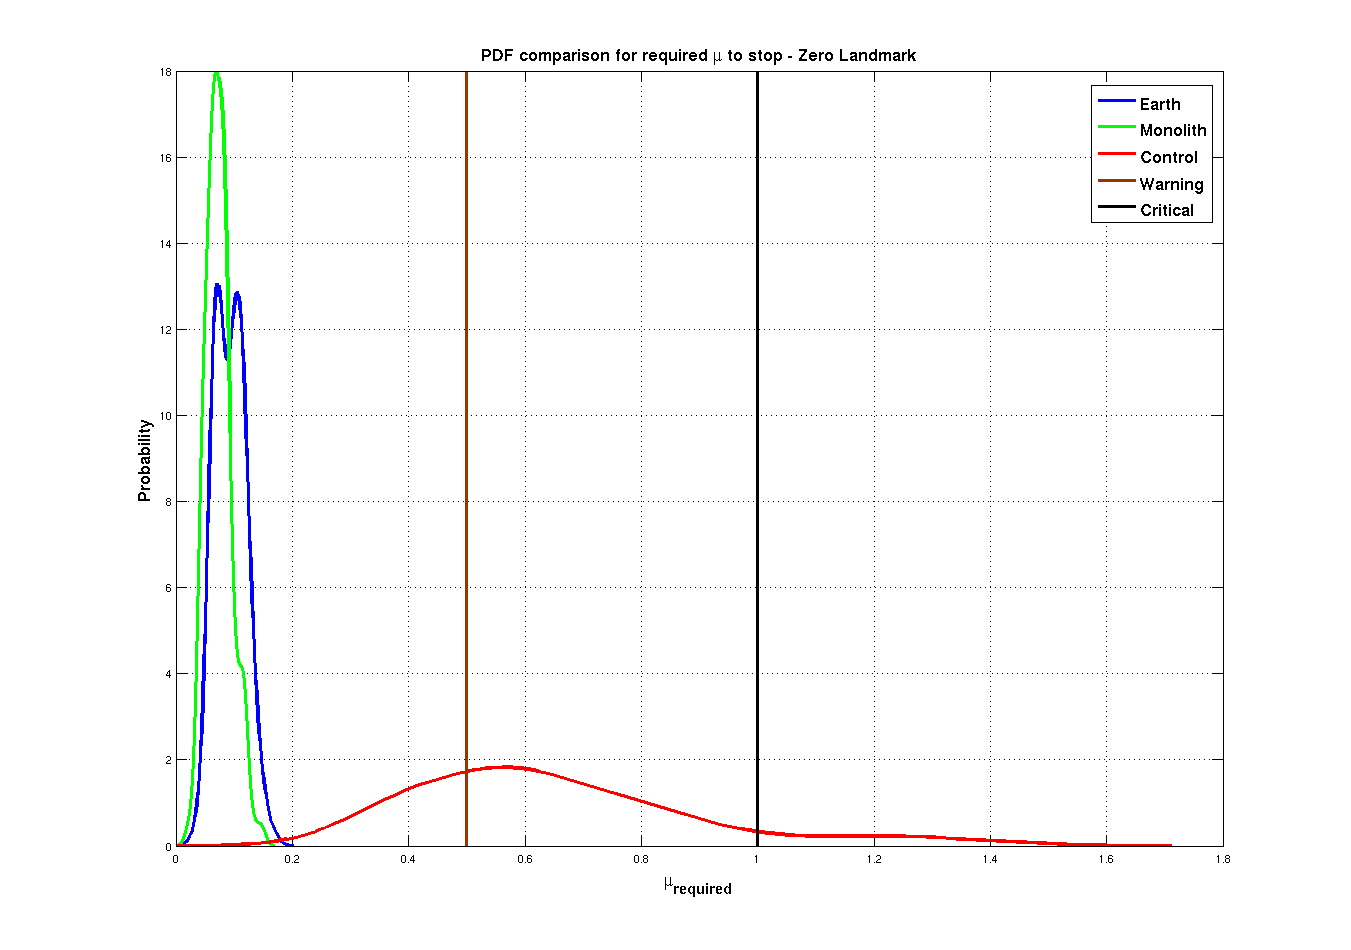
\includegraphics[width=6in]{./figs/zero_landmark_mu_distribution.png}
    \caption{Comparison of smoothed $\mu_{required}$ distributions for the zero landmark test} \label{fig:zero_mu_dist}
\end{figure}